Die Entwicklung eines Softwaresystems ist ein sich wiederholender Prozess, der sich in mehreren Phasen unterteilen lässt.
Alle Phasen beeinflüssen sich gegenseitig, sodass sie nicht unabhängig voneinander betrachtet werden können.

Die Abbildung \ref{fig:workflowCiCd} zeigt eine mögliche Aufteilung in Phasen der Entwicklung. 
\begin{figure}[H]
    \centering
    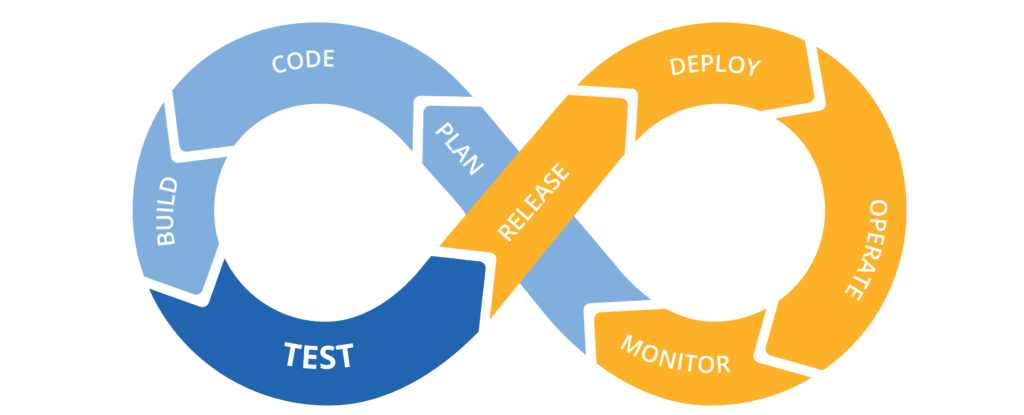
\includegraphics[width=1\textwidth]{../images/CiCD.png}
    \caption[CI/CD Pipeline]{CI/CD Pipeline \footnotemark}
    \label{fig:workflowCiCd}
\end{figure}
\footnotetext{https://blog.itil.org/2016/07/wort-zum-montag-cd-continous-delivery/}

Das Ziel ist es, die Gesamtzeit des Zyklus so minimal wie möglich zu halten, um dem Kunden die neuen Funktionalitäten schneller zur Verfügung stellen und ebenso
Bugs schneller eliminieren zu können.



Die Entwicklung von Software lässt sich in zwei übergeordnete Gruppen unterteilen:
Bevor die neue Version der Software freigegeben 
wird und nach der Freigabe der neuen Version.
Die Phasen nach der Freigabe der neuen Version lassen sich fast vollständig automatisieren 
und sind ab einem gewissen Automatisierungsgrad ressourcenschonender.
Der großte Anteil an Ressourcen wird in den ersten vier Phasen (Plan, Code, Build, Test) verbraucht, 
denn diese Aufgaben lassen sich schlecht bis gar nicht automatisieren. 

Ein hoher Anteil an manuellen Prozessen, wie z.B. Testen, Erstellen, führt in der Softwareentwicklung 
zu längeren Zykluszeiten. Es ist bereits zu Beginn des Projektes sinnvoll, Möglichkeiten von Testautomatisierungen zu betrachten.

% Und wenn man am Anfang des Projektes schlechte Entscheidungen trifft, 
% die das automatisierte Testen erschweren oder durch die schlechte Struktur 
% des Programms das Hinzufügen der neuen Funktionalität deutlich schwieriger macht, 
% wird man deutlich mehr Ressourcen gebrauchen, um das gleiche Ziel zu ereichen als wenn man das nicht gemacht hätte.

In dieser Arbeit werden Entscheidungen erläutert, 
welche bereits in den Phasen ``Plan'' und ``Code'' getroffen werden können.
Das Ziel ist die Gesamtqualität der Software zu verbesseren bei 
gleichbleibendem oder geringerem personellen Aufwand. Als Beispiel dient die Entwicklung eines OCPP Servers.